\section{Defects and dopants}\label{sec:7.4}

A phosphorus atom in silicon binds its fifth electron by \SI{45.6}{meV}, a twenty-fifth of the gap. Dark matter of \SI{13}{keV} carries enough kinetic energy to set that electron free, where the gap of the perfect crystal needs \SI{0.333}{MeV} (\cref{sec:1.3}). A carbon--hydrogen complex in the same crystal, the T center, emits light at \SI{935}{meV}, and a quarter of its photons leave without exciting a single phonon. And a silicon atom struck with a few tens of eV leaves its site for good, storing several eV in the vacancy and the interstitial it leaves behind. Defects therefore enter a dark-matter experiment in two roles: as targets with their own low thresholds, and as final states or readouts of an energy deposit. Each is built from formalism already in hand. The shallow donor is the hydrogenic envelope of \cref{sec:4.9} with the valley masses of \cref{sec:3.3}, the color center is the displaced oscillator of \cref{sec:5.6}, and the displacement threshold is a property of the energy surface of \cref{sec:5.1}.

\subsection{Shallow donors}

An atom from group V on a silicon site, such as phosphorus, arsenic or antimony, uses four of its five valence electrons in the bonds. The fifth is bound to the ion core and its one extra positive charge, in a hydrogenic donor level just below the conduction band, built from conduction-band states. An impurity of this kind is a \emph{donor}; a group-III atom such as boron, one electron short, binds a hole instead and is an \emph{acceptor}. Both bind their carrier weakly, because the host screens the Coulomb attraction by the static dielectric constant $\varepsilon_0$ and the carrier moves with the band mass $m^*$ rather than $m_e$.

The hydrogen atom with these two substitutions already sets the scale. \Cref{app:D.23} derives the envelope equation of Kohn and Luttinger~\cite{kohn1955theory} and~\cite[Chap.~4]{yu2010fundamentals}. The donor potential varies slowly on the scale of the lattice and mixes only conduction states within $\sim 1/a^*$ of a band minimum $\vect{k}_j$. The donor state is then the Bloch function at the minimum modulated by an envelope,
\begin{equation}
  \psi(\vect{r}) \simeq F_j(\vect{r})\,\psi_{c\vect{k}_j}(\vect{r}) , \qquad
  \Bigl[-\frac{\partial_x^2 + \partial_y^2}{2m^*_\perp} - \frac{\partial_z^2}{2m^*_\parallel} - \frac{\alpha}{\varepsilon_0 r}\Bigr]F_j(\vect{r}) = -E_{\mathrm{b}}^{\mathrm{D}}\,F_j(\vect{r}) ,
  \label{eq:7.4-EMT}
\end{equation}
with $z$ along the axis of the valley and $E_{\mathrm{b}}^{\mathrm{D}}$ the \emph{donor binding energy}, measured down from the conduction-band minimum. This is \emph{effective-mass theory}. It is the Wannier--Mott equation \cref{eq:4.9-envelope} with two changes. The electron is bound to a fixed ion rather than to a hole, which makes the mass the band mass and not a reduced mass. And the mass is a tensor, because the valleys of silicon are ellipsoids (\cref{sec:3.3}).

\begin{keyresult}[Effective-mass donor levels]
For an isotropic mass $m^*$ the solution of \cref{eq:7.4-EMT} is hydrogenic, with the \emph{effective Bohr radius} $a^*$,
\begin{equation}
  E_{\mathrm{b}}^{\mathrm{D}} = \frac{m^*\alpha^2}{2\varepsilon_0^2} = \frac{m^*/m_e}{\varepsilon_0^2}\,\mathrm{Ry} , \qquad
  a^* = \frac{\varepsilon_0}{m^*\alpha} = \varepsilon_0\,\frac{m_e}{m^*}\,a_0 ,
  \label{eq:7.4-hydrogenic}
\end{equation}
and excited levels at $E_{\mathrm{b}}^{\mathrm{D}}/n^2$ below the band edge.
\end{keyresult}
With $\varepsilon_0 = 11.7$ and masses of a few tenths of $m_e$, the binding is tens of meV and the orbit tens of \si{\angstrom}, several lattice constants. The assumption behind \cref{eq:7.4-EMT}, an envelope spread over many cells, is then satisfied, which makes the estimate self-consistent. For silicon the estimate brackets the answer without giving it: the transverse mass $m^*_\perp = 0.191\,m_e$ puts the binding at \SI{19.0}{meV} and $a^* = \SI{32.4}{\angstrom}$, the longitudinal mass $m^*_\parallel = 0.916\,m_e$ at \SI{91.0}{meV} and \SI{6.8}{\angstrom}.

The anisotropic problem has one parameter, the mass ratio $\gamma_m = m^*_\perp/m^*_\parallel = 0.209$. In units of the transverse Rydberg $\mathrm{Ry}^*_\perp = m^*_\perp\alpha^2/2\varepsilon_0^2 = \SI{18.98}{meV}$ and radius $a^*_\perp = \SI{32.4}{\angstrom}$, the variational envelope of Kohn and Luttinger, a hydrogen $1s$ function squeezed along the heavy axis, binds the electron by $E_{\mathrm{b}}^{\mathrm{D}} = 1.564\,\mathrm{Ry}^*_\perp = \SI{29.7}{meV}$, with the radii $r_\perp = \SI{24.3}{\angstrom}$ across the valley axis and $r_\parallel = \SI{14.0}{\angstrom}$ along it (\cref{eq:D.23-Si}). The orbit is an oblate spheroid, flattened along the heavy direction, where the electron is less mobile, and the binding lies between the two isotropic values, closer to the light one, because two of the three directions are light. The full spectrum of \cref{eq:7.4-EMT} needs a numerical solution. Scaling $z$ by $\gamma_m^{1/2}$ makes the kinetic energy isotropic and turns the Coulomb potential into $-2/[r\,(1 - (1 - \gamma_m)\cos^2\theta)^{1/2}]$ in these units. Expanding that angular factor in Legendre polynomials, and the envelope in spherical harmonics of fixed $m$ and parity, leaves a set of coupled radial equations, which we solve on a grid. The ground state comes out at $1.566\,\mathrm{Ry}^*_\perp = \SI{29.7}{meV}$, so the variational envelope is within \num{0.002} $\mathrm{Ry}^*_\perp$ of the exact effective-mass ground state. The excited states are labeled by their hydrogenic parents; the anisotropy splits each $np$ level into $np_0$, with the node across the valley axis, and $np_\pm$. \Cref{fig:7-donor} shows them.

\begin{figure}[t]
  \centering
  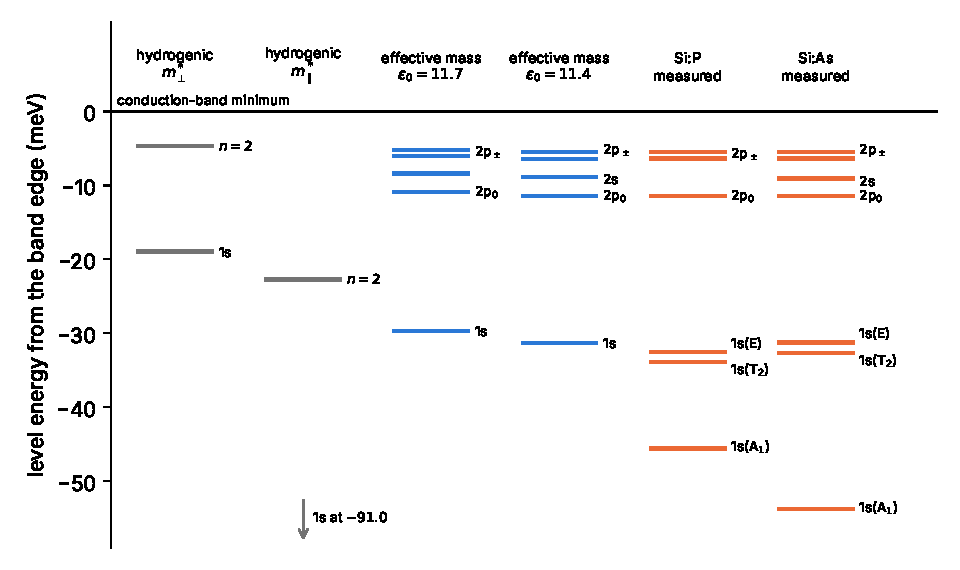
\includegraphics[width=\linewidth]{figures/ch07/fig7_4.pdf}
  \caption{Bound levels of a shallow donor in silicon, measured from the conduction-band minimum (meV). Gray: the hydrogenic model, \cref{eq:7.4-hydrogenic}, with $\varepsilon_0 = 11.7$ and the transverse mass $0.191\,m_e$ ($1s$ at \SI{19.0}{meV}) or the longitudinal mass $0.916\,m_e$ ($1s$ at \SI{91.0}{meV}, off the scale), each with its $n = 2$ level. Blue: the effective-mass equation \cref{eq:7.4-EMT} with both masses, solved numerically (coupled radial equations in spherical harmonics after scaling $z$ by $\gamma_m^{1/2}$, $l \le 14$), for $\varepsilon_0 = 11.7$ (room temperature) and 11.4 (liquid-helium temperature); from the top, $3p_0$, $2p_\pm$, $2s$, $2p_0$ and $1s$. Orange: measured levels of phosphorus and arsenic donors~\cite[Fig.~1]{vinh2008silicon}. The $p$ levels agree with effective-mass theory at $\varepsilon_0 = 11.4$ to \SI{0.4}{\percent}; the $1s$ level splits into $A_1$, $T_2$ and $E$ states, and the $A_1$ ground state lies below the effective-mass value by \SI{14}{meV} for phosphorus and \SI{22}{meV} for arsenic.}
  \label{fig:7-donor}
\end{figure}

The measured spectra test the theory state by state~\cite[Fig.~1]{vinh2008silicon}. The $p$ levels of phosphorus and arsenic agree with each other to \SI{0.02}{meV}: $2p_0$ at 11.48 and \SI{11.50}{meV}, $2p_\pm$ at \SI{6.40}{meV} for both. They do not depend on the chemistry of the donor, as effective-mass theory says they should. With $\varepsilon_0 = 11.7$, however, the theory puts them \SI{5}{\percent} too shallow, at 10.92 and \SI{6.09}{meV}. Since every level of \cref{eq:7.4-EMT} scales as $1/\varepsilon_0^2$, the measured $2p_\pm$ fixes $\varepsilon_0 = 11.7\times(6.09/6.40)^{1/2} = 11.4$. It is the value of the static constant at liquid-helium temperature, where donor spectra are taken, that calculations of donor levels use~\cite{faulkner1969higher,smith2017ab}, \SI{2.6}{\percent} below the room-temperature 11.7. With 11.4, effective-mass theory puts $2p_0$, $2p_\pm$ and $3p_0$ at 11.51, 6.42 and \SI{5.49}{meV}, within \SI{0.4}{\percent} of the measured 11.48, 6.40 and \SI{5.47}{meV}, and the $1s$ state at \SI{31.3}{meV}, the value Faulkner obtained~\cite{faulkner1969higher,smith2017ab}. The $p$ envelopes vanish at the donor site and never see the ion core.

The ground states are another matter. Phosphorus binds its electron by \SI{45.59}{meV}~\cite{jagannath1981linewidths}, arsenic by \SI{53.76}{meV}~\cite[Fig.~1]{vinh2008silicon}, and antimony by \SI{42.7}{meV}~\cite[Table~3]{claes2025accurate}, all deeper than \SI{31.3}{meV} and different from one another. The difference lies near the core. Within a lattice constant of the donor the screening by $\varepsilon_0$ is incomplete, and the potential carries the chemistry of the ion; the envelope equation replaces both by $-\alpha/\varepsilon_0 r$. The $1s$ envelope is largest exactly there, and the potential that \cref{eq:7.4-EMT} leaves out shifts it. This shift is the \emph{central-cell correction}.

The central cell also lifts a degeneracy that the effective-mass equation leaves intact. Silicon has six valleys, on the $\langle100\rangle$ axes, and each carries its own envelope, rotated with its axis; at the order of \cref{eq:7.4-EMT}, any combination $\sum_jc_jF_j\psi_{c\vect{k}_j}$ is a ground state, sixfold degenerate without spin. The short-range part of the donor potential couples the valleys, because a potential concentrated in one cell has Fourier components at the large momenta $\vect{k}_j - \vect{k}_{j'}$ between them. The donor site has the symmetry of a regular tetrahedron, the point group $T_d$, which leaves three matrix elements, $\Delta_0$ within a valley, $\Delta_{\mathrm{g}}$ between opposite valleys and $\Delta_{\mathrm{f}}$ between perpendicular ones. The six states split into a singlet $A_1$, a doublet $E$ and a triplet $T_2$. These are the standard names of the irreducible representations of $T_d$: each label says how a set of states transforms under the rotations and reflections of the tetrahedron, and here it fixes the degeneracy, one, two or three. The levels lie at
\begin{equation}
  E_{A_1} = \Delta_0 + \Delta_{\mathrm{g}} + 4\Delta_{\mathrm{f}} , \qquad
  E_E = \Delta_0 + \Delta_{\mathrm{g}} - 2\Delta_{\mathrm{f}} , \qquad
  E_{T_2} = \Delta_0 - \Delta_{\mathrm{g}} ,
  \label{eq:7.4-vo}
\end{equation}
relative to the effective-mass level (\cref{eq:D.23-vo}). In the $A_1$ state all six valleys add in phase at the donor site; it has the largest density on the core and an attractive central cell lowers it most. This \emph{valley-orbit splitting} is what the measured spectra show: the phosphorus $1s$ level is a singlet at \SI{45.59}{meV}, with the triplet $T_2$ at \SI{33.89}{meV} and the doublet $E$ at \SI{32.58}{meV}, close to the effective-mass value~\cite[Fig.~1]{vinh2008silicon}. The central-cell correction is a property of the $s$-like ground state, and a large one, a third of the binding of phosphorus.

The donor's size sets the density at which it stays a single donor. The \emph{defect density} $\nd_{\mathrm{D}}$, the number of donors (or of any defect) per unit volume, has to be small enough that orbits do not overlap, $\nd_{\mathrm{D}}a^{*3} \ll 1$. The spheroid of radii $r_\perp$, $r_\perp$ and $r_\parallel$ has a volume of \SI{3.5e-20}{cm^3}, and one donor per orbit means $\nd_{\mathrm{D}} \approx \SI{3e19}{cm^{-3}}$. In a lightly doped crystal, with $\nd_{\mathrm{D}} = \SI{e15}{cm^{-3}}$, donors sit \SI{100}{nm} apart and each is an isolated hydrogen atom of the crystal. At higher densities the electrons hop between donors and form an impurity band, and the isolated-donor picture fails before the orbits touch, at the Mott metal--insulator transition.

Acceptors are bound by similar amounts, tens of meV in silicon, but their effective-mass problem is harder. The valence maximum is degenerate, with heavy and light holes and a split-off band (\cref{sec:3.3}), and \cref{eq:7.4-EMT} becomes a set of coupled equations for several envelopes, the same complication that the heavy--light mixing brings to excitons (\cref{sec:4.9}). Donors are the cleaner case, and we keep to them.

Effective-mass theory is the computational method of choice for shallow donors, because no supercell is large enough to hold the envelope. An orbit of radius \SI{2.4}{nm} spans thousands of atoms, and a supercell calculation of the donor (\cref{app:E.10}) has to extrapolate in its size. It also inherits the error of its functional, magnified: a semilocal functional spreads the donor electron too far and binds phosphorus by only \SI{19.2}{meV} after extrapolation, against the measured \SI{45.6}{meV}~\cite[Table~3]{claes2025accurate}. What a supercell supplies well is the potential within a cell or two of the core. Combined with the envelope equation, in multivalley effective-mass theory, that potential gives the central-cell correction and the valley-orbit splitting, which is the division of labor that \cref{app:D.23} sets up.

\begin{workedexample}{The binding of phosphorus in silicon}\label{we:7-sip}
We compare the effective-mass binding of a phosphorus donor with the measured \SI{45.59}{meV} and extract the valley-orbit matrix elements, with the masses $m^*_\perp = 0.191\,m_e$ and $m^*_\parallel = 0.916\,m_e$ of \cref{tab:3-materials}.

\emph{Units.} With $\varepsilon_0 = 11.7$, $\mathrm{Ry}^*_\perp = 0.191\times\SI{13606}{meV}/11.7^2 = \SI{18.98}{meV}$, $a^*_\perp = 11.7\times\SI{0.529}{\angstrom}/0.191 = \SI{32.4}{\angstrom}$ and $\gamma_m = 0.209$.

\emph{Effective-mass ground state.} The variational envelope of \cref{app:D.23} binds the electron by \SI{29.7}{meV}, and the numerical solution of \cref{eq:7.4-EMT} gives $1.566\,\mathrm{Ry}^*_\perp$, also \SI{29.7}{meV}. At the liquid-helium value $\varepsilon_0 = 11.4$, which the $p$ levels require, $\mathrm{Ry}^*_\perp = \SI{20.00}{meV}$ and the effective-mass $1s$ level lies at \SI{31.3}{meV}.

\emph{Central-cell correction.} The measured ground state is $\SI{45.59}{meV} - \SI{31.3}{meV} = \SI{14.3}{meV}$ deeper, \SI{31}{\percent} of the binding. The measured binding itself leans on the theory: the spectroscopy measures transitions, and the absolute ground-state energy follows by adding the effective-mass binding of a high $p$ state, \SI{3.12}{meV} for $3p_\pm$, to the measured $1s(A_1) \to 3p_\pm$ line~\cite{smith2017ab}. The $p$ levels can bear that weight, as \cref{fig:7-donor} shows.

\emph{Valley-orbit matrix elements.} Taking the effective-mass level $-\SI{31.3}{meV}$ as the reference, the three measured $1s$ levels of phosphorus, $A_1$ at $-45.59$, $T_2$ at $-33.89$ and $E$ at \SI{-32.58}{meV}, sit at $-14.29$, $-2.59$ and \SI{-1.28}{meV}. \Cref{eq:7.4-vo} gives $E_{A_1} - E_E = 6\Delta_{\mathrm{f}}$, so $\Delta_{\mathrm{f}} = -13.01/6 = \SI{-2.17}{meV}$; then $\Delta_0 + \Delta_{\mathrm{g}} = E_E + 2\Delta_{\mathrm{f}} = \SI{-5.62}{meV}$ and $\Delta_0 - \Delta_{\mathrm{g}} = E_{T_2} = \SI{-2.59}{meV}$, so that $\Delta_0 = \SI{-4.10}{meV}$ and $\Delta_{\mathrm{g}} = \SI{-1.51}{meV}$. All three are negative, as an attractive core requires, and the coupling between perpendicular valleys is the larger of the two intervalley terms. The $E$ and $T_2$ states lie only 1.3 and \SI{2.6}{meV} below the effective-mass value, and the $A_1$ state takes \SI{14.3}{meV}, because only $A_1$ collects all six valleys in phase at the core.

\emph{Size.} The variational envelope of \cref{app:D.23} has $|F(0)|^2 = 1/(\pi r_\perp^2r_\parallel)$, with the radii $r_\perp = \SI{24.3}{\angstrom}$ and $r_\parallel = \SI{14.0}{\angstrom}$ found above. The volume of one silicon atom is $a^3/8$, with the lattice constant $a = \SI{5.43}{\angstrom}$, and the probability of finding the electron within it around the donor is $|F(0)|^2a^3/8 = (\SI{5.43}{\angstrom})^3/(8\pi\times24.3^2\times\SI{14.0}{\angstrom^3}) = \num{7.7e-4}$ per valley envelope. The central cell is a small region of the orbit, and still it moves the ground state by a third: the potential there is that of an unscreened ion, many eV deep.

\emph{Kinematics.} Dark matter can ionize the donor if $\tfrac12\mchi v_{\mathrm{max}}^2 \ge E_{\mathrm{b}}^{\mathrm{D}}$, that is for $\mchi \ge 2\times\SI{45.59}{meV}/\num{7.023e-6} = \SI{13.0}{keV}$, twenty-six times lighter than the \SI{0.333}{MeV} of the silicon gap. At threshold the momentum transfer is $\mchi v_{\mathrm{max}} = \SI{34.4}{eV}$. The envelope spreads over momenta up to $1/r_\perp = \SI{81}{eV}$ across the valley axis and $1/r_\parallel = \SI{141}{eV}$ along it, so $qr_\perp \approx 0.42$: the dark matter that can just ionize the donor transfers momenta that the bound electron has. In the language of \cref{sec:1.3}, the donor is a good kinematic match to dark matter of a few tens of keV.
\end{workedexample}

\subsection{Color centers}

The T center of silicon emits at \SI{935}{meV}, \SI{1326}{nm} in the telecommunications O band, and the nitrogen--vacancy center of diamond at \SI{1.945}{eV}, \SI{637}{nm}. Both lines are sharp, and both sit on a broad band of lower-energy light. Defects of this kind are called \emph{color centers}, after the F centers that color the alkali halides. Their levels lie deep in the gap, and their electrons are confined within a cell or two of the defect, unlike the donor electron of the previous subsection. A localized electron that changes its state exerts large forces on the few atoms around it. The nuclei settle at different positions in the ground and the excited state, and an optical transition, which is fast compared with the nuclear motion, leaves them displaced from their new equilibrium. This is the displaced oscillator of \cref{sec:5.6}, and color centers are where its parameters are measured.

The \emph{configuration-coordinate diagram} draws the two Born--Oppenheimer surfaces of \cref{sec:5.1}, one for each electronic state, along the single coordinate $Q$ that connects their minima. With $Q$ mass-weighted, as $\Delta Q = M^{1/2}\Delta x$ in \cref{sec:5.6}, and one effective mode of energy $\omega_0$ that is the same in both states,
\begin{equation}
  E^{\mathrm{ad}}_{\mathrm{g}}(Q) = \tfrac12\omega_0^2Q^2 , \qquad
  E^{\mathrm{ad}}_{\mathrm{e}}(Q) = E_{\mathrm{ZPL}} + \tfrac12\omega_0^2(Q - \Delta Q)^2 , \qquad
  S_{\mathrm{HR}} = \tfrac12\omega_0\Delta Q^2 .
  \label{eq:7.4-cc}
\end{equation}
The \emph{zero-phonon-line energy} $E_{\mathrm{ZPL}}$ is the difference between the two minima, the energy of the transition that leaves the vibrational state unchanged, and the Huang--Rhys factor $S_{\mathrm{HR}}$ measures the displacement in units of the zero-point spread of the mode. A vertical transition from the ground minimum lands $\tfrac12\omega_0^2\Delta Q^2 = S_{\mathrm{HR}}\omega_0$ above the excited minimum, so absorption peaks near $E_{\mathrm{ZPL}} + S_{\mathrm{HR}}\omega_0$; emission from the relaxed excited state peaks near $E_{\mathrm{ZPL}} - S_{\mathrm{HR}}\omega_0$, and the lattice takes up the relaxation energy $S_{\mathrm{HR}}\omega_0$ each way. At $T = 0$ the emission lines at $E_{\mathrm{ZPL}} - p\,\omega_0$ carry the Poisson weights $\ee^{-S_{\mathrm{HR}}}S_{\mathrm{HR}}^p/p!$ of \cref{eq:5.6-FC}, and the zero-phonon line carries
\begin{equation}
  w_{\mathrm{ZPL}} = \ee^{-S_{\mathrm{HR}}} .
  \label{eq:7.4-zpl}
\end{equation}
A real center couples to a continuum of crystal modes and to a few local modes of its own atoms; $S_{\mathrm{HR}}$ is then the sum of the factors of all the modes, the replicas merge into a sideband, and the zero-phonon weight is still $\ee^{-S_{\mathrm{HR}}}$ (\cref{sec:5.6}). The color-center literature calls this weight the Debye--Waller factor of the line; in this book that name belongs to $\ee^{-2W}$ of \cref{eq:5.6-W}, and we write \emph{zero-phonon fraction}.

The \emph{T center} is a pair of carbon atoms sharing one silicon site, with a hydrogen atom on one of them~\cite{bergeron2020characterization}. Its ground state has one unpaired electron. Its luminescent state is a bound exciton: a second electron pairs with the first into a singlet, and a hole is bound to the negatively charged complex by only \SI{34.78(15)}{meV}, out of a total pair binding of about \SI{235}{meV}. The hole binding comes from the series of excited hole levels seen in photoluminescence excitation, extrapolated to the ionization limit of the hole~\cite[Sect.~IV]{bergeron2020characterization}. The loosely bound hole is a shallow, effective-mass-like particle, while the electrons are deep and localized. Measured on an ensemble in isotopically pure $^{28}$Si between 1.4 and \SI{4.2}{K}, the exciton lives \SI{0.94}{\micro s}, and \SI{23}{\percent} of the emitted photons are in the zero-phonon line~\cite{bergeron2020silicon}.

The \emph{nitrogen--vacancy center} of diamond is a substitutional nitrogen next to a vacant site along $[111]$. In its negative charge state six electrons occupy orbitals built from the dangling bonds around the vacancy, and its spin-triplet ground state is optically read out at room temperature~\cite[Sect.~1.1]{doherty2013nitrogen}. A fit of its measured emission band at \SI{8}{K} returns $S_{\mathrm{HR}} = 3.85 \pm 0.05$ with an effective phonon energy of \SI{64}{meV}~\cite[Sects.~3 and~4.3]{alkauskas2014first}.

\Cref{fig:7-cc} draws both centers in units of their own phonon energy, where the diagram depends on $S_{\mathrm{HR}}$ alone. The T center's minima are displaced by $(2S_{\mathrm{HR}})^{1/2} = 1.7$ zero-point units, the nitrogen--vacancy center's by 2.8. That difference becomes a factor of ten in the zero-phonon weight. The measurements are taken at temperatures where the coupled modes are empty: at \SI{4.2}{K}, a phonon of \SI{10}{meV} has a thermal occupation of $\ee^{-\omega/T} = \num{1e-12}$, and the zero-temperature weights of \cref{eq:7.4-zpl} apply.

\begin{figure}[t]
  \centering
  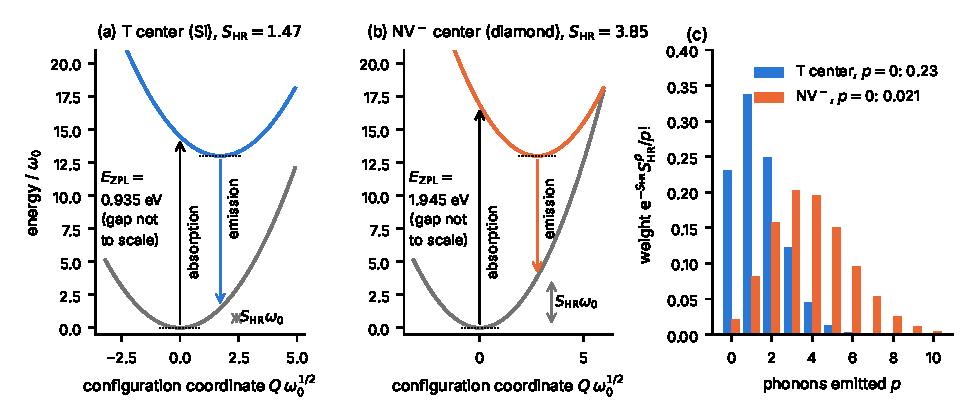
\includegraphics[width=\linewidth]{figures/ch07/fig7_5.pdf}
  \caption{Configuration-coordinate diagrams of (a) the T center in silicon, $E_{\mathrm{ZPL}} = \SI{0.935}{eV}$, $S_{\mathrm{HR}} = 1.47$ (from the measured zero-phonon fraction 0.23~\cite{bergeron2020silicon}), and (b) the negatively charged nitrogen--vacancy center in diamond, $E_{\mathrm{ZPL}} = \SI{1.945}{eV}$, $S_{\mathrm{HR}} = 3.85$~\cite{alkauskas2014first}. Each center is modeled by one effective mode of energy $\omega_0$, the same in both electronic states, in the Condon approximation; energies are in units of $\omega_0$ (\SI{64}{meV} for the nitrogen--vacancy center) and the coordinate in units of $\omega_0^{-1/2}$, \cref{eq:7.4-cc}. Gray: ground-state surface; colored: excited state, drawn with a reduced gap $E_{\mathrm{ZPL}}$ (not to scale). Arrows: vertical absorption from the ground minimum and emission from the excited minimum; the double arrow is the relaxation energy $S_{\mathrm{HR}}\omega_0$. (c) Zero-temperature weights of the emission lines with $p$ phonons emitted, $\ee^{-S_{\mathrm{HR}}}S_{\mathrm{HR}}^p/p!$; the zero-phonon line is $p = 0$.}
  \label{fig:7-cc}
\end{figure}

Comparing \cref{eq:7.4-zpl} with a luminescence spectrum needs one correction. The rate of spontaneous emission into a line of energy $E$ grows as $E^3|\vect{d}|^2$, with $\vect{d}$ the transition dipole, so a luminescence spectrum counts photons with the Franck--Condon weight times $E^3$~\cite[Eq.~(2)]{alkauskas2014first}. The sideband lies at lower energy and is suppressed by this factor, and the zero-phonon line takes a larger share of the photons than of the Franck--Condon weight:
\begin{equation}
  \frac{\text{photons in the zero-phonon line}}{\text{all photons}} = \frac{\ee^{-S_{\mathrm{HR}}}E_{\mathrm{ZPL}}^3}{\sum_p\ee^{-S_{\mathrm{HR}}}S_{\mathrm{HR}}^p(E_{\mathrm{ZPL}} - p\,\omega_0)^3/p!} ,
  \label{eq:7.4-photon}
\end{equation}
in the single-mode model. The correction is of order $3S_{\mathrm{HR}}\omega_0/E_{\mathrm{ZPL}}$, large when the relaxation energy is a sizable fraction of the line energy.

Computing these numbers is a supercell problem. $E_{\mathrm{ZPL}}$ is the difference of two total energies, each at its own relaxed geometry, with the excited state obtained by constraining the occupations of the defect orbitals; $S_{\mathrm{HR}}$ follows from the displacement between the two geometries projected on the vibrational modes, $S_{\mathrm{HR}} = \sum_k\omega_k\Delta Q_k^2/2$. A hybrid functional in a 512-atom cell puts the T-center line at \SI{985}{meV}, \SI{50}{meV} above the measurement~\cite{dhaliah2022first}, and the converged Huang--Rhys factor of the nitrogen--vacancy center is 3.67 against the measured 3.85~\cite[Sects.~4.2 and~4.3]{alkauskas2014first}.

\begin{workedexample}{Zero-phonon fractions}\label{we:7-zpl}
We compute the zero-phonon fractions of the T center and the nitrogen--vacancy center and check the second against its measured photon count.

\emph{T center.} Through \cref{eq:7.4-zpl}, the measured photon fraction 0.23 means $S_{\mathrm{HR}} = -\ln0.23 = 1.47$. The weights of the lines with 0, 1, 2 and 3 phonons are 0.23, 0.34, 0.25 and 0.12 (\cref{fig:7-cc}c): one photon in four is in the zero-phonon line, and one in three has emitted exactly one phonon. Read through \cref{eq:7.4-photon}, the photon fraction slightly overstates the Franck--Condon weight. The bound on the correction, $3S_{\mathrm{HR}}\omega_0/E_{\mathrm{ZPL}}$ with $\omega_0$ at most the \SI{64}{meV} of the silicon optical phonon (\cref{sec:5.3}), is $3\times1.47\times0.064/0.935 = 0.30$, so the photon count shifts $S_{\mathrm{HR}}$ by at most 0.30. The true Huang--Rhys factor lies between 1.47 and about 1.8, and the zero-phonon weight between 0.23 and 0.17.

\emph{Nitrogen--vacancy center.} With $S_{\mathrm{HR}} = 3.85$, \cref{eq:7.4-zpl} gives $w_{\mathrm{ZPL}} = \ee^{-3.85} = 0.021$, ten times less than the T center. The line with three phonons is the strongest, at 0.20. The relaxation energy is $S_{\mathrm{HR}}\omega_0 = 3.85\times\SI{64}{meV} = \SI{0.246}{eV}$, so absorption peaks near \SI{2.19}{eV} and emission near \SI{1.70}{eV}, a Stokes shift of \SI{0.49}{eV}.

\emph{The photon check.} In \cref{eq:7.4-photon}, with $\omega_0/E_{\mathrm{ZPL}} = 0.064/1.945 = 0.0329$, the Poisson average of $(1 - 0.0329\,p)^3$ is
\begin{equation*}
  1 - 3(0.0329)S_{\mathrm{HR}} + 3(0.0329)^2(S_{\mathrm{HR}} + S_{\mathrm{HR}}^2) - (0.0329)^3(S_{\mathrm{HR}} + 3S_{\mathrm{HR}}^2 + S_{\mathrm{HR}}^3) = 0.677 ,
\end{equation*}
from the first three moments of the Poisson distribution. The photon fraction is then $0.0213/0.677 = 0.031$. The measured share of the zero-phonon line in the emission is \num{0.032}~\cite[Sect.~3]{alkauskas2014first}. Taken at face value, $-\ln0.032$ would give $S_{\mathrm{HR}} = 3.44$, an underestimate by 0.4 that the single-mode model attributes entirely to the $E^3$ weighting.

\emph{Detection fraction.} A detector that reads a color center through its zero-phonon line collects a quarter of the T center's photons and three percent of the nitrogen--vacancy center's. The rest come out in the sideband, spread over several phonon energies below the line, where a narrow filter rejects them together with the background.
\end{workedexample}

\subsection{Displacement thresholds and Frenkel pairs}

A silicon atom struck along $\langle111\rangle$ with \SI{12.5}{eV} can leave its site for good; struck along $\langle100\rangle$, it needs \SI{20}{eV}~\cite[Table~IV]{holmstrom2008threshold}. Below these energies the atom swings out, hands its energy to its neighbors and returns. The difference between the two outcomes is a statement about the energy surface $E^{\mathrm{ad}}(u)$ of \cref{sec:5.1}. The perfect crystal is its lowest minimum, but the surface has many other local minima, separated from it by barriers of several eV. A \emph{vacancy} is an empty lattice site. An \emph{interstitial} is an extra atom between the sites; in silicon it can sit at the tetrahedral or the hexagonal interstitial site or share a site with a lattice atom as a split $\langle110\rangle$ dumbbell. An atom moved from its site into an interstitial position leaves a vacancy behind, and the two together are a \emph{Frenkel pair}. Each configuration costs a formation energy, the height of its minimum above that of the perfect crystal. Density-functional calculations put the isolated vacancy at 3.4 to \SI{3.9}{eV}, the interstitials at 4.7 to \SI{5.8}{eV}, and the most stable close Frenkel pair, a tetrahedral interstitial \SI{4.7}{\angstrom} from its vacancy, at 6.8 to \SI{7.5}{eV}~\cite[Table~III]{holmstrom2008threshold}. A cheaper minimum exists without any vacancy: the \emph{bond defect}, a local rearrangement of bonds, at 2.6 to \SI{3.0}{eV}.

The \emph{displacement threshold energy} $E_{\mathrm{d}}(\hat{\vect{r}})$ is the smallest kinetic energy that, given to one atom in the direction $\hat{\vect{r}}$, leaves the crystal in a minimum other than the perfect one once the motion has died out,
\begin{equation}
  E_{\mathrm{d}}(\hat{\vect{r}}) = \min\bigl\{E_R :\ \text{the trajectory on } E^{\mathrm{ad}} \text{ from } (E_R, \hat{\vect{r}}) \text{ ends in a defect}\bigr\} .
  \label{eq:7.4-Ed}
\end{equation}
It is not the formation energy of the pair it creates, and it is always larger. The struck atom must squeeze between its neighbors, over a barrier that lies on its path and not at the end points. It loses energy to every atom it pushes. And if it stops too close to its own vacancy, the pair recombines and the crystal returns to its minimum. $E_{\mathrm{d}}$ therefore depends on the direction, through the open and closed channels of the lattice, and on the path of the whole collision. It is computed by molecular dynamics: a single trajectory on $E^{\mathrm{ad}}$ for each direction and energy, repeated over many directions (\cref{app:E.11}).

For silicon, density-functional molecular dynamics finds the lowest threshold, \SI{12.5}{eV}, along $\langle111\rangle$, where the struck atom pushes its neighbor into the tetrahedral site in a short replacement sequence; \SI{20}{eV} along $\langle100\rangle$; and \SI{36}{eV} for a Frenkel pair averaged over all directions~\cite[Table~IV]{holmstrom2008threshold}. Electron-irradiation experiments see damage set in at $12.9 \pm \SI{0.6}{eV}$~\cite{loferski1958radiation}, in agreement with the minimum. In most directions a bond defect forms at a lower energy than a Frenkel pair, and the average threshold for a defect of either kind is \SI{24}{eV}~\cite[Table~IV]{holmstrom2008threshold}. Which number is quoted depends on what is counted: a count of vacant and doubly occupied lattice sites sees the Frenkel pair but not the bond defect. The classical Stillinger--Weber potential, used for the large statistical scans, overshoots the density-functional thresholds along $\langle111\rangle$ by 4 to \SI{6}{eV}~\cite[Sect.~IV]{holmstrom2008threshold}, and its thresholds range from 17.5 to \SI{63.5}{eV} over all directions~\cite{kadribasic2018directional}.

The threshold is not the energy that stays in the crystal. A close Frenkel pair stores \SIrange{6.8}{7.5}{eV}, about half of the minimum threshold and a fifth of the average one; the rest of the recoil energy becomes heat within picoseconds. The stored energy is invisible to a calorimeter that measures the heat. It is a missing part of the deposit, and \cref{sec:19.4} turns this into the defect fraction of a recoil and the bounds that calibration data put on it. For dark matter, only heavy enough particles can reach these thresholds at all. By \cref{eq:1.3-ERmax}, with the silicon nuclear mass $M = \SI{26.16}{GeV}$ and $v_{\mathrm{max}} = \num{2.650e-3}$, a recoil of \SI{12.5}{eV} needs $\mchi \ge \SI{0.153}{GeV}$, and one of \SI{36}{eV} needs \SI{0.26}{GeV}. Since $E_{\mathrm{d}}$ depends on the direction of the recoil relative to the crystal axes, the rate of defect creation near threshold carries the direction of the dark-matter wind, a handle for directional detection~\cite{kadribasic2018directional}.

\subsection{Defects as targets and readouts}

A shallow donor is a target in its own right, with the threshold and the kinematic match of \cref{we:7-sip}. Its weakness is the number of electrons. A donor density of \SI{e15}{cm^{-3}} is five parts in $10^{9}$ of the valence electrons of silicon, \SI{2.0e23}{cm^{-3}}, and the interaction with the bound electron is screened by the same $\varepsilon_0$ that makes it shallow. The rate requires the response of the donor to the dark-matter operators, with its valleys and central cell, which \cref{sec:16.5} derives.

A color center is a target with a level inside the gap and a readout with an optical line. As a target, the T center needs $\mchi \ge 2\times\SI{0.935}{eV}/v_{\mathrm{max}}^2 = \SI{0.266}{MeV}$, below the \SI{0.333}{MeV} of the silicon gap, because its excitation sits \SI{0.24}{eV} below the band edge. The momentum at threshold is $2E_{\mathrm{ZPL}}/v_{\mathrm{max}} = \SI{0.71}{keV}$, and a transition at that momentum needs states localized to about $1/\SI{0.71}{keV} = \SI{2.8}{\angstrom}$, which the deep levels of the center are. The nitrogen--vacancy center needs \SI{0.554}{MeV} and \SI{1.47}{keV}. As a readout, the zero-phonon fraction sets how many of a center's photons survive a narrow filter (\cref{we:7-zpl}), and the spins of both centers can be polarized and read optically. As a final state, a color center can be created by a nuclear recoil, by a displacement or by the capture of a vacancy, and the threshold $E_{\mathrm{d}}$ sets where that begins (\cref{sec:16.6}).

A displaced atom, finally, is a long-lived final state. The Frenkel pair or the bond defect left by a recoil persists as long as its barriers allow. At \SI{10}{mK} the Boltzmann factor for crossing a barrier of \SI{0.1}{eV} is $\ee^{-1.2\times10^5}$, and only tunneling or the phonons of a later event move the defect.

\section*{Summary}

The Coulomb interaction does not act on spin, yet it couples spins, and in NiO it orders them below \SI{523}{K} (\cref{sec:7.1}). At low energy only the spins remain, coupled by the Heisenberg model, and in NiO one exchange constant, the measured $J_2 = \SI{19.01}{meV}$ between next-nearest nickel neighbors, sets the scale. In an antiferromagnet the exchange creates spin deviations in pairs, a bosonic Bogoliubov transformation removes the pair terms, and the dispersion becomes linear, with a measured maximum of ${\sim}\SI{117}{meV}$ in NiO. Density-functional values of $J_2$ spread from 11 to \SI{27}{meV}, and that spread is the theory uncertainty for a magnet without neutron data. A dark-matter particle that couples to the electron spin acts through the spin density $\vect{s}_e(\vect{q})$, and its one-magnon response follows from the Bogoliubov coefficients.

Phonon exchange makes electrons near the Fermi surface attract each other, with the dimensionless strength $\mathcal{N}_{\mathrm{F}}V_{\mathrm{BCS}} = \lambda_{\mathrm{ep}}$, reduced by the quasiparticle residue and the Coulomb pseudopotential (\cref{sec:7.2}). The excitations of the BCS state are Bogoliubov quasiparticles of energy $(\xi_{\vect{k}}^2 + \Delta_{\mathrm{BCS}}^2)^{1/2}$, and a probe that conserves the electron number creates them in pairs, so the threshold is $2\Delta_{\mathrm{BCS}}$. Independent quasiparticles, however, do not conserve charge; the conserving response of the Nambu formalism removes the defect through the phase mode of the condensate and satisfies the density Ward identity. For aluminum the measured critical temperature fixes $\Delta_{\mathrm{BCS}} = \SI{0.179}{meV}$, a threshold of \SI{0.36}{meV} and a threshold mass of \SI{0.10}{keV}.

Near a point where two bands nearly touch, the $\vect{k}\cdot\vect{p}$ expansion becomes a Dirac Hamiltonian, with the velocity $v_{\mathrm{D}}$ in place of the speed of light and the half-gap $\Delta_{\mathrm{D}}$ in place of the mass (\cref{sec:7.3}). A cone with $v_{\mathrm{D}} > v_{\mathrm{max}}$ cannot be excited by scattering at any mass, while a slow cone opens the target to light particles: \SI{8.0}{keV} for ZrTe$_5$-like parameters. The Dirac electrons screen on top of a background dielectric constant $\varepsilon_{\mathrm{bg}}$, with the effective coupling $\tilde\alpha = \alpha/(\varepsilon_{\mathrm{bg}}v_{\mathrm{D}})$, and a gapless cone has no screening length.

Defects put levels inside the gap of silicon itself (\cref{sec:7.4}). Effective-mass theory binds every shallow donor by \SI{31.3}{meV} at the liquid-helium dielectric constant 11.4, and the central-cell correction of the $s$-like ground state, \SI{14.3}{meV}, brings phosphorus to its measured \SI{45.6}{meV}, which opens silicon to dark matter of \SI{13}{keV}. A color center couples its electronic transition to local vibrations, and the measured zero-phonon fraction $\ee^{-S_{\mathrm{HR}}} = 0.23$ of the T center of silicon means $S_{\mathrm{HR}} = 1.47$. A recoiling atom that receives more than the displacement threshold, \SI{12.5}{eV} along $\langle111\rangle$ in silicon, leaves a Frenkel pair or a bond defect that stores energy no calorimeter sees. \Cref{chap:8} gathers the responses of all these targets, and those of the earlier chapters, into one framework for the rate.
